\documentclass[a4paper]{article}
\newcounter{QuestionNumber}
\setcounter{QuestionNumber}{1}

\newcommand{\Q}{
\textbf{Question \theQuestionNumber)}
\stepcounter{QuestionNumber}
}
\usepackage{amsmath,amssymb,graphicx,subcaption,caption}
\usepackage{enumitem}
\usepackage[margin=1in]{geometry}
\usepackage{lipsum}
 \renewcommand{\familydefault}{\rmdefault}
\setlength{\parindent}{0pt}
\setlength{\parskip}{1em}
\begin{document}
\Large
\begin{center}
In the name of beauty

The 10th problem set solution of Optical Networks course

\hrulefill
\end{center}
%\section*{HW9: Dynamic Optical Networks}
%\begin{enumerate}
%\item

\Q

We must sort the wavelengths in descending order, where we obtain

80Gbps - 60Gbps - 40Gbps - 40Gbps - 40Gbps - 30Gbps

Starting from the first wavelength, the 80Gbps must be accomodated in a wavelength, 60 and 40 be put in another, whereas the next two 40s are placed in another wavelength and finally, the last 30Gbps demand must occupy another wavelength, totally consuming 4 wavelengths.

\Q

%Consider the following network. Grooming connections (GCs) are matched according to the table below. The wavelength line rate is 40Gbps and the optical reach is 500km. State the number of regenerations before and after the grooming operation. Draw groomed paths on the network.
%
%\begin{center}
%
\includegraphics[width=120mm]{grooming_bus}
%\end{center}
%
%\begin{table}[h]
%\centering
%\Large
%\begin{tabular}{|c|c|c|c|}
%\hline
%&Source&Destination&Requested rate
%\\\hline
%GC1&B&D&2*10G
%\\\hline
%GC2&C&E&2*10G
%\\\hline
%GC3&D&E&1*10G
%\\\hline
%GC4&A&B&2*10G
%\\\hline
%\end{tabular}
%\end{table}

Without grooming, the connections B-D and C-E require a regeneration each, since they traverse beyond optical reach. When grooming is performed, the demands GC2 and GC3 over link DE and the demands C-E and B-D are multiplexed, each of which on a line-rate. With this paradigm, no regeneration is required since electrical grooming is automatically capable of regenerating signals.


\Q

%Consider the IP-over-OTN-over-Optical nodal architecture of Fig(a). Assume that 50\% of the traffic that enters the node remains in the optical layer; i.e., it optically bypasses both the OTN and IP layers. Of the traffic that is dropped from the optical layer, 50\% of it can bypass the IP layer; i.e., it is only groomed by the OTN switch. The remainder is delivered to the IP router. What cost ratio between the IP ports and the OTN ports justifies this architecture from a cost basis, as compared to the IP-over-Optical nodal architecture of Fig(b), where all of the non-optical-bypass traffic is delivered to the IP router? (Assume that all of the costs of the IP routers and OTN switches are in the ports. Assume that the OTN network-side ports and OTN client-side ports have the same cost.)

Let each port of the IP router and the OTN switch costs $C_\text{IP}$ and $C_\text{OTN}$, respectively. Containing $n$ such ports, an IP router or an OTN switch would cost totally as $nC_\text{IP}$ and $nC_\text{OTN}$ respectively.

If a 50\% of the total of entered traffic is dropped, we assume that providing that ratio of traffic requires an IP router (or an OTN switch) with exactly $m$ ports. The architecture on left would then cost for $mC_\text{IP}$. On the other hand, for the right-side architecture, the OTN switch must contain $m$ network ports, connecting to the ROADM, and $m/2$ client ports, connecting to the IP router. The latter must hold since 50\% of the dropped traffic is forwarded to the IP router. This imposes that the IP router must also contain exactly $m/2$ ports, leading to a total cost of
$$
\frac{m}{2}C_\text{IP}+\frac{m}{2}C_\text{OTN}+mC_\text{OTN}
=\frac{m}{2}C_\text{IP}+\frac{3m}{2}C_\text{OTN}.
$$
Implication on economical superiority of the right-side architecture on the one on left yields
$$
\frac{m}{2}C_\text{IP}+\frac{3m}{2}C_\text{OTN}<mC_\text{IP},
$$
which gives
$$
C_\text{OTN}<\frac{1}{3}C_\text{IP}.
$$
As a matter of fact, the IP routers are more expensive than OTN router, since they must be capable of handling all the layers below 3, rather than below layer 2 as is the case in OTN switches.


%\begin{figure}[h]
%\centering
%\begin{subfigure}{0.49\textwidth}
%\centering
%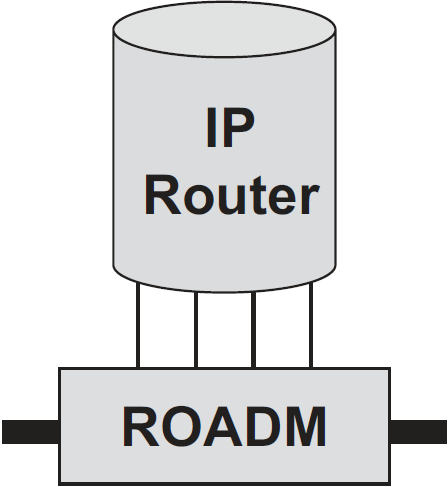
\includegraphics[width=30mm]{IP_router}
%\end{subfigure}
%\begin{subfigure}{0.49\textwidth}
%\centering
%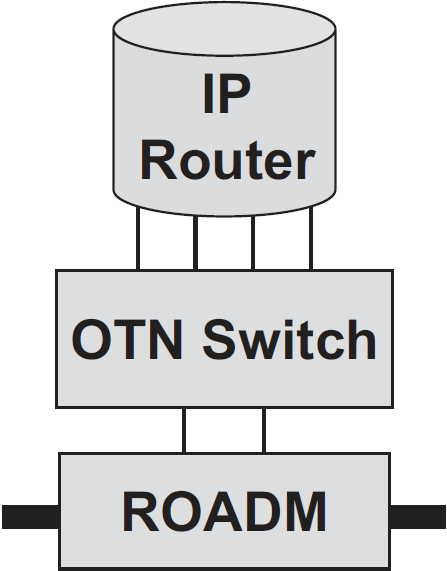
\includegraphics[width=30mm]{IP_OTN}
%\end{subfigure}
%\end{figure}

\Q

%Assume that 135 (identical and independent) services are multiplexed onto a 50GHz wavelength. Each service can be represented by an ON/OFF model, where a service is ON with probability 0.6. When the service is ON, the requested bit rate is 125 Mb/s, deploying PM-QPSK (i.e. four bits per symbol is sent) and sinc pulse shaping.

PM-QPSK maps each symbol to four bits, hence the bandwidth required for each service is 0.5GHz. Since the line-rate is 50GHz, we can place 100 such services adjacently without interference (however, this scenario is far from reality since even close services on spectrum do interfere, but we neglect it here for simplicity)

\begin{enumerate}[label=\alph*-]
\item
The desired event takes place when more that 100 concurrent services share the mediafor transmission. In terms of equations, we have
$$
P=\sum_{k=101}^{135}\binom{135}{k}(0.6)^k(0.4)^{135-k}
\approx 2.1642\times 10^{-4}
$$
\item
$$
np=135\times .0.6=81\equiv 40.5\text{GHz}\equiv 81\%
$$
\item
If $m$ such services exist in total, we must have at least $\frac{10}{0.5}=20$ concurrent services to experience collisions. The desired probability is
$$
P=\sum_{k=21}^m\binom{m}{k}(0.6)^k(0.4)^{m-k}
$$
which must be less than $\approx 2.1642\times 10^{-4}$, hence $m=22$.
%Next, consider the scenario where these same services are multiplexed onto 10GHz wavelengths. How many services can be multiplexed onto one 10GHz wavelength such that the probability that the intended offered load exceeds the wavelength bit rate is no higher than $P$?
\item
$$
0.6m=0.6\times 22= 13.2\equiv 5.6\text{GHz}\equiv 56\%
$$
%With this number of services on a 10GHz wavelength, on average, how full is the wavelength?
%\item
%What is the statistical multiplexing gain in the 100 Gb/s scenario versus the 10 Gb/s scenario (for the level of P calculated above)?
\end{enumerate}

%\end{enumerate}
\end{document}


